\documentclass[12pt,a4paper]{article}
\usepackage[width=.75\textwidth]{caption}
\usepackage{graphicx}
\usepackage{authblk}
\usepackage{amsmath}
\usepackage{amsfonts}
\usepackage{braket}
\usepackage{epigraph}
%\usepackage{mathrsfs}
\usepackage[mathscr]{euscript}
\usepackage[top=2cm, bottom=2cm, left=2cm, right=2cm]{geometry}
\usepackage{fancyhdr}

\setlength{\epigraphwidth}{0.8\textwidth}

% \pagestyle{fancy}
\begin{document}

%title and author details
\title{Field Theoretic Perspective on Thrust of an Accelerating Frame}
\author[1]{Kevin Player\footnote{kplayer@andrew.cmu.edu}}

\maketitle

\epigraph{The Unruh effect tells us that what we call particles is really just a matter of perspective.}{Lee Smolin}

\abstract{We analyze the quantum field theoretic framework where Unruh radiation was first described, interpreting acceleration as a driving source influencing the field. By conceptualizing this source as thrust, we provide a more intuitive mechanism for understanding radiation in accelerating frames.  Using the equivalence principle, we extend this framework to Hawking radiation as well, demonstrating how a common source-response relationship manifests in accelerating frames.}


\section{Introduction}

We begin by introducing the preliminaries, concepts, and notations for discussing quantum field theory in an accelerating frame, with a focus on positive frequency modes in Rindler spacetime. Building on this foundation, we introduce the concept of field-theoretic driving sources and extend the formalism using the Fourier transform to analyze these sources as a combination of emission and absorption terms. This framework allows us to develop a field-theoretic interpretation of thrust as a driving source for particle production in non-inertial frames. By examining the dynamics of these driving sources, we derive the Unruh vacuum expectation value, highlighting its connection to acceleration and quantum field theory. Finally, we interpret thrust as Unruh radiation and leverage the equivalence principle to explore its role in Hawking radiation, establishing a conceptual link between thrust, external sources, and the emergence of thermal radiation in an accelerating frame.

Much of the content, including notation and conventions, is directly adapted from the overview in \cite{Frodden}, the foundational work in \cite{unruh}, and the detailed treatment in \cite{beisert}. Consistent with these references, our focus is restricted to the free scalar field, which suffices to elucidate the Unruh effect.

\section{Rindler and Minkowski Modes Review}

Let $\hbar$ = $c$ = 1 and consider a uniform linear acceleration in $1+1$ dimensional spacetime. The full $1+3$ dimensional case does not add anything to the discussion, so without loss of generality we stick to the dimensions time $t$ and space $z$ where the boost is taking place.  The massless Klein-Gordon equation 

\begin{equation}
  \Box \phi = \frac{\partial^2 \phi}{\partial t^2} - \frac{\partial^2 \phi}{\partial z^2} = 0,
 \label{massless-wave-eq}
\end{equation}
has solutions which we describe using a basis  $u = -t + z$ and $v = -t - z$, the null coordinates along the light cone.  Any function of purely $u$, $f(u)$, is made up of modes that are constant on $v$.  That is they are given by a 1-dimensional Fourier expansion
\begin{equation}
  f(u) = \frac{1}{2\pi} \int{e^{i p_u u} \hat{f}(p_u) dp_u}.
\end{equation}
supported on $p_v = 0$.  The same is true for $v$, $g(v)$, $p_v$, and $\hat{g}(v)$ supported on $p_u = 0$.  The full space of solutions to equation (\ref{massless-wave-eq}) are combinations of $f$ and $g$, linear combinations of $\hat{f}(p_u) \delta(p_v)$ and $\hat{g}(p_v) \delta(p_u)$.  These are supported on the massless shell $E = \pm p$.  A basis of solutions are the ``Minkowski modes''
\begin{equation}
  \frac{1}{\sqrt{2\omega_k (2\pi)^{n-1}}} e^{i(k x - \omega_k t)}
\end{equation}
where $\omega^2 = k^2$, covering both the positive and negative frequency cases $\omega = \pm k$.

\begin{figure}[h]
\centering
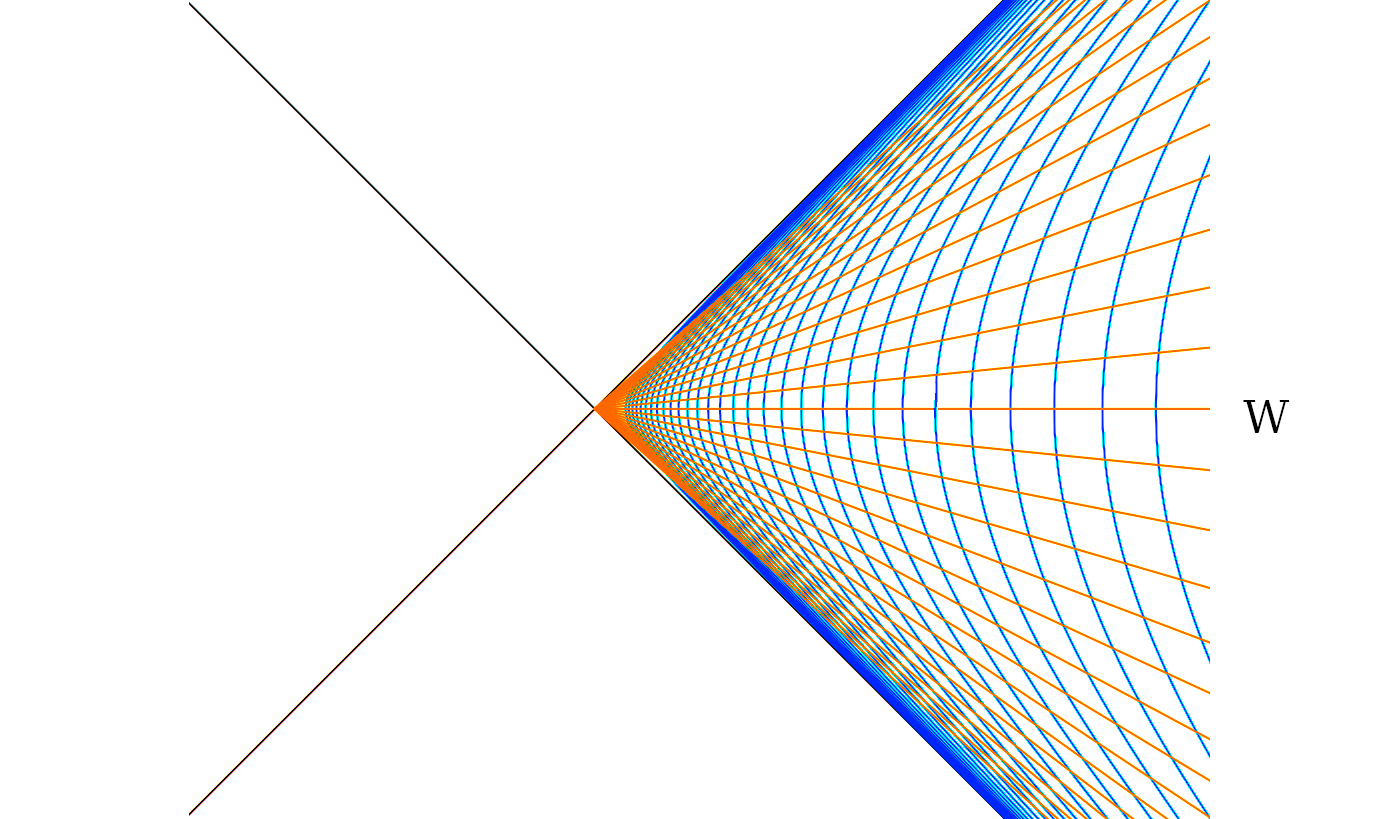
\includegraphics[scale=0.2]{rindler_w.png}
\caption{Rindler wedge $W$ on the right.}
\label{rindlerw}
\end{figure}

The following notations and results for the rest of this section are taken from \cite{Frodden}. Let $W$ be the $z>|t|$ Rindler ``wedge'' with coordinates
\begin{equation}
  t = \frac{1}{a}e^{a\xi}\sinh{(a\eta)}
\label{sinh}
\end{equation}
\begin{equation}
z = \frac{1}{a}e^{a\xi}\cosh{(a\eta)}
\end{equation}
where $a>0$ is an acceleration parameter (see Figure \ref{rindlerw}). The massless Klein-Gordon equation in Rindler coordinates is
\begin{equation}
  \Box \phi = e^{-2a \xi}(-\partial_\eta^2 + \partial_\xi^2) \phi = 0.
\end{equation}
which has a basis of solutions 
\begin{equation}
 r_k = \frac{1}{\sqrt{4 \pi \omega_k}} e^{-i(\omega_k \eta -k \xi)}
\end{equation}
for each wave number $k$ and positive frequency $\omega_k = |k|$.  These ``Rindler modes'' do not immediately extend to the entire $(x,t)$-plane but are confined to the Rindler wedge $W$. 

Consider the analytic functions on the entire $(x,t)$-plane
\begin{equation}
h^{(u)}_k = \frac{e^{\frac{\pi \omega_k}{2a}} {(au)}^{\frac{i\omega_k}{a}}}{ \sqrt{2\sinh\left(\frac{\pi\omega_k}{a}\right)}}
\end{equation}
\begin{equation}
h^{(v)}_k = \frac{e^{\frac{\pi \omega_k}{2a}} {(av)}^{\frac{i\omega_k}{a}}}{ \sqrt{2\sinh\left(\frac{\pi\omega_k}{a}\right)} }
\end{equation}
These two functions are functions of $u$ and $v$ respectively, and so are solutions to equation (\ref{massless-wave-eq}).  Each $r_k$ can be extended to the entire plane as
\begin{equation}
e^\frac{\pi\omega_k}{2a} h^{(u)}_k - e^{-\frac{\pi\omega_k}{2a}} h^{(v)}_k  = \sqrt{2 \sinh \left({\frac{\pi\omega_k}{a}}\right)} r_k
\end{equation}

Let $c_k^{(1)}$ and $c_k^{(2)}$ be annihilation and creation operators for the positive and negative frequency Minkowski modes respectively.  Define
\begin{equation}
  b_k = \frac{1}{\sqrt{2 \sinh\left(\frac{\pi \omega_k}{a}\right)}} \left( e^{\frac{\pi\omega_k}{2a}} c_k^{(1)} + e^{-\frac{\pi\omega_k}{2a}} c_{-k}^{(2) \dagger} \right).
\end{equation}
Then the number of particles that an accelerating observer will see in the Minkowski vacuum $\ket{0_M}$ is seen to be 
\begin{equation}
\label{radeq}
\braket{n} = \bra{0_M} b_k^\dagger b_k \ket{0_M} = \frac{1}{e^{\frac{2 \pi \omega_k}{a}}-1}
\end{equation}
which is usually interpreted as (Unruh) radiation.

\section{Fourier Transform of the Sources}
We will take several Fourier transforms to study the various modes and set up for some
integrals.  Let $\phi$ be a free scalar field in the flat $1+1$ dimensional Minkowski spacetime.  We will consider $h^{(u)}_k$ and $h^{(v )}_k$ as driving $W$-event horizon sources
\begin{equation}
\label{ab}
\rho = \alpha h^{(u)}_k + \beta h^{(v)}_k.
\end{equation}
with non-negative real convex combination $\alpha + \beta = 1$.
The drivers $h^{(u)}_k$ and $h^{(v)}_k$ are functions $f(u)$ of the past $W$-horizon and $g(v)$ of the future $W$-horizon respectively.  Both generate excitations, which we identify with absorption and emission thrusts respectively.


The sources can originate from a coupling term, $\rho \phi$, added to the free scalar Lagrangian.
\begin{equation}
\mathscr{L}_{driven} = \mathscr{L}_{free} + \rho\phi 
\end{equation}
where
\begin{equation}
  \mathscr{L}_{free} = -\frac{1}{2} \partial^\mu \phi \partial_\mu \phi - \frac{1}{2} \phi^2.
\end{equation}
This leads to an inhomogeneous Klein-Gordon equation
\begin{equation}
\Box  \phi = \rho
\end{equation}
as presented in \cite{beisert}\footnote{In \cite{beisert} it is assumed that the source is only active for a finite amount of time.  We let $\rho$ be active for all time.  The argument in \cite{beisert} seem to be adaptable to $\rho$.}

We want to integrate $\rho$ on shell in momentum space, which for a massless source is the positive energy part of the massless shell.  The two positive energy ``horizons'' border $p_u <= 0$ and $p_v <= 0$, see Figure \ref{masslessshell}.  Proceeding to take the Fourier transform of the function $f(u)$\footnote{WLOG since $g(v)$ is of the same form.}, we drop $p_u$ to just $p$ for the time being to increase legibility.  We will continue to assume that $\omega_k$ and $a$ are positive. Define the kernel

\begin{equation}
  A = e^{-i p u} (au)^\frac{i\omega_k}{a} du
\end{equation}
and then we have
\begin{equation}
\label{finalnorm}
  \hat{f}(\_u) =  \frac{e^{\frac{\pi \omega_k}{2a}}}{\sqrt{2 \sinh \left({\frac{\pi\omega_k}{a}}\right)}}  \int_{-\infty}^\infty A
\end{equation}
where $L=\int_{-\infty}^0 A$ and $R=\int_0^\infty A$ are the left and right sides of the total integral $L + R$.

\begin{figure}[h]
\centering
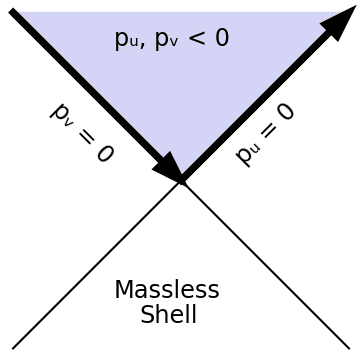
\includegraphics[scale=0.5]{massless_shell.png}
\caption{Massless shell is when $p_u$ = $p_v$ = 0}
\label{masslessshell}
\end{figure}


We rewrite the integrals using a complex changes of variables, $s$ = $ipu$, and contour integrals.

\begin{figure}[h]
\centering
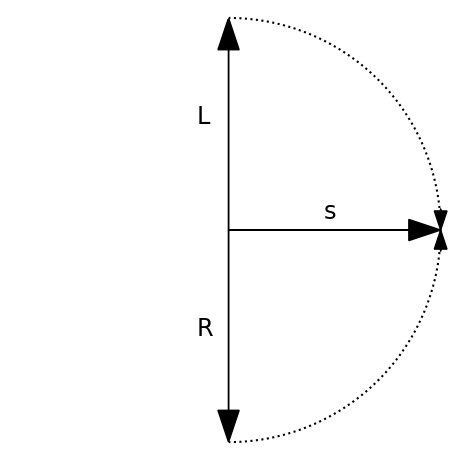
\includegraphics[scale=0.3]{contour.png}
\caption{Using contours with large radius we convert the $L$ integral that goes to $i\infty$, and the $R$ integral that goes to $-i\infty$, to integrals with $s$ going to real $\infty$.}
\label{fig:x cubed graph}
\end{figure}


The $L$ integral for real $p<0$ is
\begin{equation}
\begin{split}
  L(p) & = -\int_0^{i\infty} \left(\frac{ias}{-p}\right)^\frac{i\omega_k}{a} \left(\frac{i}{-p}\right)ds \\
  & = \frac{-i}{a} \left(\frac{a}{-p}\right)^{\frac{i\omega_k}{a} + 1} \int_0^\infty \left(is\right) ^ \frac{i\omega_k}{a} e^{-s} ds \\
  & = \frac{-i}{a} \left(\frac{a}{-p}\right)^{\frac{i\omega_k}{a} + 1} \Gamma\left(\frac{i\omega_k}{a} + 1\right) e^{-\frac{\pi \omega_k}{2a}} \\
  & = \frac{1}{2} \Gamma\left(\frac{i\omega_k}{a} + 1\right) e^{-\frac{\pi \omega_k}{2a}} B(p)\\
\end{split}
\end{equation}
where
\begin{equation}
B(p) = \frac{-2i}{a} \left(\frac{a}{-p}\right)^{\frac{i\omega_k}{a} + 1} 
\end{equation}
is as shown.  This is using a large radius contour which rotates the endpoint 90 degrees clockwise.

The same calculation for $R$ is done using a counter-clockwise contour this time.
\begin{equation}
\begin{split}
  R(p) = \frac{1}{2}\Gamma\left(\frac{i\omega_k}{a} + 1\right) e^{-\frac{\pi \omega_k}{2a}} B(p)
\end{split}
\end{equation}

We get back to $h_k^{(u)}$ and apply the normalization from equation (\ref{finalnorm})
\begin{equation}
\hat{h_k}^{(u)}(p_u) = \frac{e^{\frac{\pi \omega_k}{2a}}}{\sqrt{2 \sinh \left({\frac{\pi\omega_k}{a}}\right)}}  ( L(p_u) + R(p_u) )
\end{equation}
So
\begin{equation}
\label{fourier}
\begin{split}
\hat{h_k}^{(u)}(p_u) & = \frac{\Gamma\left(\frac{i\omega_k}{a} + 1\right)}{\sqrt{2 \sinh \left({\frac{\pi\omega_k}{a}}\right)}} B(p_u)\\
\hat{h_k}^{(v)}(p_v) &= \frac{\Gamma\left(\frac{i\omega_k}{a} + 1\right)}{\sqrt{2 \sinh \left({\frac{\pi\omega_k}{a}}\right)}} B(p_u)
\end{split}
\end{equation}
\section{Interpretation}
The driving source $\rho$, with mixed absorption and emission thrusts $\alpha$ + $\beta$ = 1, contribute excitations to the scalar field $\phi$. Equations (\ref{ab}) and (\ref{fourier}) let us write down the expected change of energy
\begin{equation}  
  \label{number}
  \begin{split}
    \mathbb{E}[\Delta E] &= \frac{1}{4\pi} \int{|\rho(p)|^2 dp} \\
    &= \frac{\alpha}{4\pi} \int{\left|\hat{h_k}^{(u)}(p_u)\right|^2 dp_u} + \frac{\beta}{4\pi}\int{\left|\hat{h_k}^{(v)}(p_v)\right|^2dp_v} \\
    &= \frac{\left|\Gamma\left(\frac{i\omega_k}{a} + 1\right)\right|^2}{2 \sinh \left({\frac{\pi\omega_k}{a}}\right)} \frac{1}{4\pi} \int{{\left|B(p)\right|^2} dp} \\
    &=  \frac{\left|\Gamma\left(\frac{i\omega_k}{a} + 1\right)\right|^2}{2 \pi a \sinh \left({\frac{\pi\omega_k}{a}}\right)} \int{a/|p|^2 dp}\\  
&=I(\omega_k) P
  \end{split}
\end{equation}
where the integrals are on the positive energy massless shell with contributions from $p_u$ on the left piece and $p_v$ on the right piece.  We factored out $P = \int{a/|p|^2}$ with a remaining $p$ independent positive real coefficient $I(\omega_k)$.

Without being more careful we end up with inferred problems --- The integrals do not converge at zero, where $P$ explodes.  But this infinity cancels when we compare the spectral radiances to each other, $I(\omega_{k_1}) / I(\omega_{k_2})$.

The magnitude of our Gamma function has known asymptotics \cite[Eq.~5.11.9]{NIST:DLMF}
\begin{equation}
\left|\Gamma\left(\frac{i\omega_k}{a} + 1\right) \right|^2 \sim \left(\frac{2 \pi \omega_k} {a}\right) e^{-\frac{\pi\omega_k}{a}}
\end{equation}
Plugging this into equation (\ref{number}) we find the average energy of the mode, the $1+1$ dimensional Planck distribution function, and thus recover the Unruh's radiation spectrum from a thrust driven field.
\begin{equation}
\frac{1}{P} \mathbb{E}[\Delta E] = I(\omega_k) \sim \frac{\omega_k}{e^{\frac{2 \pi \omega_k}{a}}-1}
\end{equation}
Compare this to equation (\ref{radeq}) and references \cite{unruh} and \cite{Frodden}.

\section{Conclusion and Prediction}
If the thrust required to accelerate a detector is not explicitly accounted for, it manifests instead as an apparent thermal feature of the vacuum—Unruh radiation. However, as demonstrated in this paper, Unruh radiation can be directly explained as a consequence of thrust. This perspective leads to the prediction that neither Unruh radiation nor Hawking-Bekenstein radiation should appear independently of the thrust that drives the system.

\section{Acknowledgments}
Thanks to Ben Commeau and Daniel Justice for useful discussions.

\bibliographystyle{ieeetr}
\bibliography{bibliography}

\end{document}
